\section{Diskreter Logarithmus}
	%TODO Diskreter Logarithmus
	Diskreter Logarithmus ... [TODO]
	
	\subsection{Elliptischen Kurven Grundlagen}
		In diesem Kapitel sollen nur die Grundlagen von elliptischen Kurven näher gebracht werden, um so die \textbf{E}lliptic \textbf{C}urve \textbf{C}ryptography, kurz ECC, verstehen zu können. Der Vorteil beim ECC-Verfahren im Vergleich zum RSA-Verfahren, liegt darin das die Schlüssellänge deutlich kürze ausfallen kann ohne dabei an Sicherheit zu verlieren. Ein RSA-Schlüssel mit 1024 Bit ist etwa so sicher wie ein Schlüssel aus einer elliptischen Kurve mit gerade mal ca. 160 Bit. Dazu kommt das der Rechenaufwand und Speicherbedarf beim ECC-Verfahren wesentlich geringer ist als beim RSA-Verfahren. So kann ECC in Smartcards und Mobiltelefonen genutzt werden.\cite{Information:und:Kommunikation}
				
		Um die Funktionsweise der elliptischen Kurven in ihrer vollen Breite und Tiefe zu verstehen ist dafür eine sehr komplexe Mathematik notwendig. Innerhalb dieser Seminararbeit kann dieses Thema nicht Breiter und Tiefer durchleuchtet werden und es sei ihr auf die folgende Literatur verwiesen: \cite{Information:und:Kommunikation} und \cite{Kryptographie:und:IT-Sicherheit}.
		
		Eine Elliptische Kurve ist eine ebene Kurve wie in Abbildung~\ref{ABBILDUNG_elliptischenKurveAddition} gezeigt. Sie wird durch eine Gleichung der Form: $y^2 = x^3 + ax +b$ beschrieben. Damit ist eine Menge Z aller Punkte P(x, y) die auf der elliptischen Kurve liegen definiert. Wichtig dabei ist das die Kurvenparameter a und b so gewählt sind das die partiellen Ableitungen nach x und nach y auf keinem Punkt der Kurve gleichzeitig null sind, dazu später mehr.
		
		Das Addieren von zwei Punkten, die auf der elliptischen Kurve liegen, ergibt wieder einen Punkt welcher ebenfalls auf der Kurve liegt.\cite{Information:und:Kommunikation} Mit Addition ist das Verknüpfen von zwei Punkten gemeint, man könnte es auch als Multiplikation bezeichnen. In beiden fällen hat es nichts mit den bekannten Operationen auf Zahlen zu tun. Das Addieren von zwei Punkten ist vielmehr geometrisch definiert, siehe dazu auch Abbildung~\ref{ABBILDUNG_elliptischenKurveAddition}:
		
		\begin{figure}
			\centering
			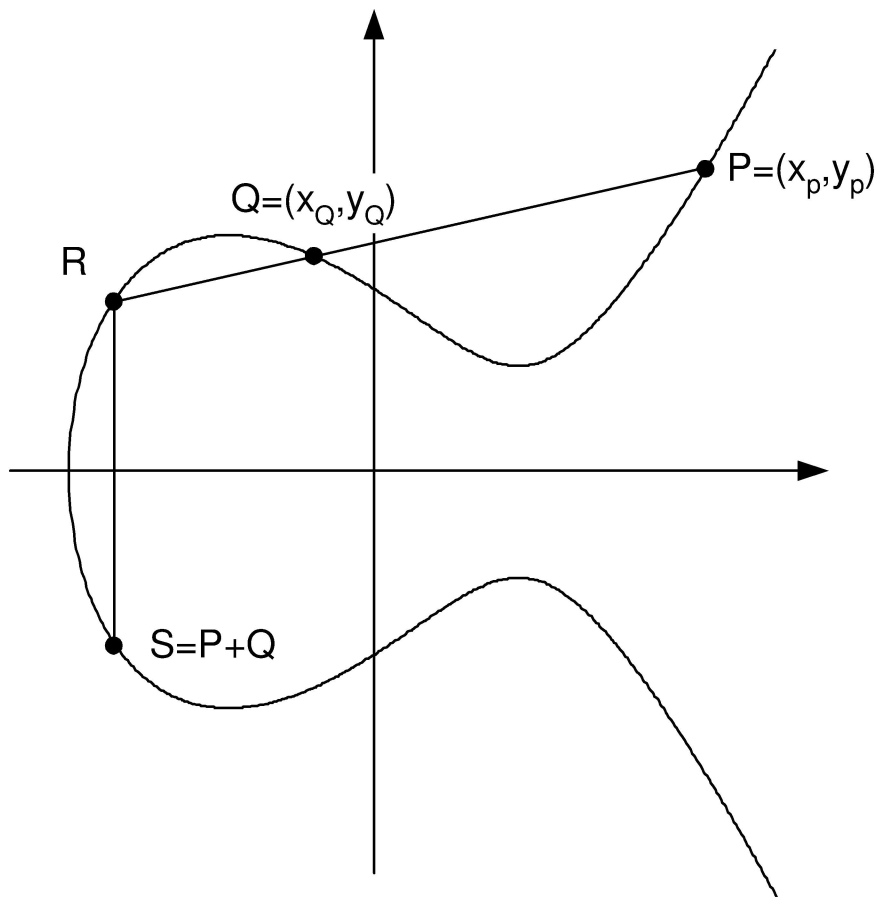
\epsfig{file=includes/images/ElliptischeKurveAddition.PNG, height=3in, width=3in}
			\caption{Addition von zwei Punkten auf einer elliptischen Kurve~\cite{Information:und:Kommunikation}}
			\label{ABBILDUNG_elliptischenKurveAddition}
		\end{figure}
		
		\begin{quote}
			\begin{defi}
				Durch die gegebenen Punkte P und Q wird eine Gerade gelegt, welche die Kurve in einem dritten Punkt R schneidet. Dieser wird anschließend an der x-Achse 
				gespiegelt. Als Ergebnis erhält man den Punkt S, welcher als Addition von P und Q bezeichnet wird.\cite{Information:und:Kommunikation}
			\end{defi}
		\end{quote}
		
		Die so definierte Addition ist kommutativ, zur Erinnerung: P + Q = Q + P. Nicht für alle elliptischen Kurven kann eine Addition von Punkten durchgeführt werden. Wie oben bereits erwähnt dürfen die partiellen Ableitungen nach x und nach y auf keinem Punkt der Kurve gleichzeitig null sein. Anders ausgedrückt die Kurve darf sich nicht selbst schneiden, ansonsten kann die Additionsoperation nicht für beliebige Punkte durchgeführt werden.
		Zusätzlich muss beachtet werden, dass bei einer Addition von zwei Punkten die nachfolgenden Spezialfälle auftreten können\cite{Information:und:Kommunikation}:
		
		\begin{itemize}
			\item Wenn für die beiden zu Addierenden Punkten Q = P gilt, wird die Tangente an der Kurve im Punkt P verwendet. Dabei entsteht der der Schnittpunkt mit der Kurve in R und durch Spiegelung resultiert daraus S = P + P = 2P.
			\item Sollten die X-Koordinaten beider zu addierender Punkte gleich sein, so dass (Q\myTiefstellen{X} = P\myTiefstellen{X}) gilt, entsteht eine vertikale Gerade und die Kurve wird kein weiteres mal geschnitten. Für diesen Fall wird die elliptische Kurve um einen weiteren Punkt \myInftyOhne, welcher im Unendlichen liegt, ergänzt. Die Addition von Punk P mit \myInfty ist so definiert das man wiederum P als Ergebnis erhält (P + \myInfty = P). Somit ist \myInfty das neutral Element der Addition. Es gilt also: P + Q = \myInfty wenn die x-Koordinaten von P und Q gleich sind. Daraus folgt das Q das inverse Element vo P ist und es gilt: Q = -P.
		\end{itemize}
		
		Das Addieren eines Punktes P mit einem Skalar k \myin \{1, 2, 3 ...\} wird als wiederholte Addition definiert:
		
		\begin{displaymath}
			kP = P1 + P2 + ... + Pk
		\end{displaymath}
		
	\subsection{Asymmetrische Verschlüsselung mit Elliptischen Kurven}
		Um Elliptischen Kurven für Asymmetrische Verschlüsselung einsetzen zu können muss in einem endlichen Körper gerechnet werden um Rundungsfehler zu vermeiden. Bei der Addition und Multiplikation in endlichen Körpern sind diese so definiert, dass das Ergebnis immer wider ein Element des endlichem Körpers ist. Aufgrund dessen muss eine weitere Operation durchgeführt werden: $mod~|Z|$. Dies stellt sicher das der resultierende Rest ist in jedem Fall wieder ein Element aus Z ist. Für die Addition besitzt jedes Element ein inverses Element -a, damit gilt für die Subtraktion: $b - a = b + (-a)$. Bei der Multiplikation ist das inverse Element $a^{-1}$, damit gilt für die Division: $b / a = b$ \mycdot $a^{-1}$. Für ein konkretes Beispiel sei an dieser Stelle auf S. 154 - 257 in \cite{Information:und:Kommunikation} verwiesen.
		
		Um elliptische Kurven für kryptologische Anwendungsfälle zu nutzen, muss die Ordnung eines Punktes der elliptischen Kurve berechnet werden.
		
		\begin{quote}
			\begin{defi}
				Die Ordnung eines Punktes ist die Anzahl der Punkte, die durch fortwährender Addition dieses Punktes, erzeugt werden.\cite{Information:und:Kommunikation}
			\end{defi}
		\end{quote}
		
		Dazu folgendes Beispiel:
		
		\begin{displaymath}
			P + P = 2P \Rightarrow 2P +P = 3P \Rightarrow ... \Rightarrow xP + P = (x+1)P
		\end{displaymath}
				
		P ist dabei immer ein Punkt auf der elliptischen Kurve. Irgendwann ist x\myTiefstellen{i}P = \myInfty, somit kein Punkt mehr auf der Kurve, und damit hat der Punkt P die Ordnung x\myTiefstellen{i}, im weiteren verlauf als n bezeichnet.
		
		\subsubsection{Schlüsselaustausch mit elliptischen Kurven}
			Zuerst muss der Körper bestimmt werden und eine elliptische Kurve, dazu wählt man ein große Primzahl und die Kurvenparameter a und b. Weiter wird nun ein Erzeugerpunkt G vereinbart, dabei soll die Ordnung des Punktes G möglichst groß und eine Primzahl sein. A wählt eine geheime ganze Zahl n\myTiefstellen{A} welche kleiner sein muss als n und berechnet daraus den öffentlichen Schlüssel P\myTiefstellen{A} = n\myTiefstellen{A} \mycdot G. Teilnehmer B mach das gleich jeweils mit n\myTiefstellen{B} und P\myTiefstellen{B}. P\myTiefstellen{A} und P\myTiefstellen{B} können nun über eine unsichere Leitung ausgeschaut werden. Nun kann Teilnehmer A den Schlüssel K = n\myTiefstellen{A} \mycdot P\myTiefstellen{B} berechnen. B berechnet ebenfalls K mit n\myTiefstellen{B} und P\myTiefstellen{A}. So habe dabei ein und das selbe geheime K berechnet.
			
			Es folgt der Beweis das A und B wirklich das gleiche K berechnet haben müssen:
			\begin{quote}
				\begin{beweis}
					A berechnet K = n\myTiefstellen{A} \mycdot P\myTiefstellen{B}. P\myTiefstellen{B} wurde ursprünglich von Teilnehmer B berechnet mit n\myTiefstellen{B} \mycdot G. Dies kann in die Berechnung für K von A an stelle von P\myTiefstellen{B} eingesetzt werden so das daraus folgt: K = n\myTiefstellen{A} \mycdot P\myTiefstellen{B} = n\myTiefstellen{A} \mycdot (n\myTiefstellen{B} \mycdot G). Das gleiche Prinzip angewendet für die Berechnung von K durch Teilnehmer B ergibt: K = n\myTiefstellen{B} \mycdot P\myTiefstellen{A} = n\myTiefstellen{B} \mycdot (n\myTiefstellen{A} \mycdot G). Unter Berücksichtigung des Assoziativgesetzes können diese beiden Gleichungen, gleich gesetzt werden:
					
					\centering n\myTiefstellen{A} \mycdot (n\myTiefstellen{B} \mycdot G) = n\myTiefstellen{B} \mycdot (n\myTiefstellen{A} \mycdot G)
				\end{beweis}
			\end{quote}
			
			Asymmetrische Verschlüsselungsverfahren basieren auf Einwegfunktionen. Wobei es nicht allzu schwierig ist k \mycdot P zu Berechnen allerdings ist das Berechnen von k aus k \mycdot P und P sehr aufwendig. Anzumerken ist das diese aussage allerdings bis heute noch nicht bewiesen wurde.
			
	\subsection{Das Problem des diskreten Logarithmus im Detail}
		Es existiert eine Primzahl p, ein erzeugendes Element g für \myZPStern~sowie eine ganze Zahl x. Zu der diskreten Exponentialfunktion $g^x~mod~p$ gibt es die diskrete Logarithmusfunktion, die zu einem gegebenen y und g, x beschreibt. Somit ist x der diskrete Logarithmus von y zur Basis g. ($y = g^x~mod~p$) Jede Zahl aus \myZPStern~lässt sich als Potenz von g darstellen, wenn g ein erzeugendes Element von \myZPStern~ist. Ist dies nicht der Fall, so muss es nicht zu jedem $y$ \myin \myZPStern einen diskreten Logarithmus geben.~\cite{Kryptografie:in:Theorie:und:Praxis} Um das eigentliche Problem des diskreten Logarithmus zu verstehen ist es hilfreich nochmal konkret Logarithmen in \myMenge{R} mit Logarithmen in \myZPStern gegenüberzustellen. 
		
		\textbf{[TODO die beiden Gleichungen von\cite{DLP:ECDLP:Probleme:und:Loesungen} S. 11 in einer miniPage gegenüberstellen]}
		
		Die Gleichung \textbf{[TODO Nr.]} zeigt wie der Logarithmus von x zur Basis g, mit der Logarithmusfunktion berechnet werden kann. Auf diese Weise sind Gleichungen für die positiven reellen Zahlen \myMenge{R^+} immer eindeutig lösbar. Bei der Gleichung \textbf{[TODO Nr.]} wird ebenfalls mit der Logarithmusfunktion versucht den Logarithmus von 10 zu Basis 2 zu erhalten. Als Ergebnis erhält man eine Zahl die nicht in enthalten ist. Was auch nicht verwundert, da die Logarithmusfunktion $mod~11$ gar nicht berücksichtigt. Genau hier ist das grundsätzlich Problem beim diskreten Logarithmus. Es gibt keine mathematische Rechenoperation die es ermöglicht den diskreten Logarithmus in einem endlichen Körper mit nur einem Rechenschritt zu berechnen. Um dennoch eine Lösung zu erhalten, scheint das Enumerationsverfahren das naheliegendste zu sein. Hierbei werden einfach alle Werte die für $k$ in frage kommen durchprobiert. So ist die Lösung für Gleichung \textbf{[TODO Nr.]} $k = 5$. Für sehr große Gruppen, wo k Beispielsweise eine 160 Bit große Zahl ist, gibt es bis heute keine Algorithmen die den diskreten Logarithmus effizient berechnen.~\cite{DLP:ECDLP:Probleme:und:Loesungen} Es gibt allerdings eine ganze Reihe von Algorithmen die in der Lage sind den diskreten Logarithmus gezielter zu berechnen als das naive Ausprobieren. Nachfolgend soll der Baby-Step-Giant-Step-Algorithmus genauer betrachtet werden.
		
	\subsection{Baby-Step-Giant-Step-Algorithmus}
		In der Praxis ist es mit diesem Algorithmus nicht möglich eine Verschlüsselung die auf dem DLP aufbaut zu brechen. Die Komplexität diese Algorithmus liegt in $O(\sqrt[]{p-1})$ ist somit schon deutlich besser als eine naive vollständige Suche, deren Komplexität in $O(p-1)$ liegt, dennoch zu stark von der Größe der zugrundeliegenden Gruppe abhängig ist. Anzumerken ist, dieser Algorithmus ist ein sogenannter generischer Algorithmus, womit dieser für jede Gruppe funktioniert und nicht von einer speziellen Struktur der Gruppe abhängt.~\cite{Kryptografie:in:Theorie:und:Praxis}
		
		Zuerst wählt der Algorithmus eine Zahl t \myin \myMenge{N}, sodass $t < \sqrt[]{p-1}$\textbf{[TODO Größer gleich]} ist. Mit einer zweiten Zahl r ($0<r<t$)\textbf{TODO[kleiner gleich]} lässt sich die Gleichung des diskreten Logarithmus schreiben als: $x = q \cdot + r$ und lässt sich wie folgt umformen
		
		\textbf{TODO[Gleichung von Kryptographie in Theo... S. 136]}
		
		Nun müssen die zwei Zahlen r und q gesucht werden, sodass die Gleichung $y \cdot g^{-r} = g^{q \cdot t}$ gilt. Dazu werden zwei Listen angelegt und im Nachhinein werden die eintrage miteinander verglichen. 
		
		\textbf{TODO[Baby-Step Liste Giant-Steo Liste von Kryptographie in Theo... S. 136]}
		
		Sollte ein Eintrag vorhanden sein der in beiden Listen vorkommt, liefert dieser den diskreten Logarithmus x.~\cite{Kryptografie:in:Theorie:und:Praxis}
		
		\subsubsection{Baby-Step-Giant-Step Vorgehen}
			Zu erst errechnet man t mit $\sqrt[]{p-1}$. Nun werden alle baby steps benötigt, diese werden mit Gleichung \textbf{[TODO Nr.]} ermittelt:
			
			\textbf{[Gleichung von \cite{DLP:ECDLP:Probleme:und:Loesungen} S. 26 für die Baby Steps]}
			
			Die Ergebnisse von \textbf{[TODO Gleichung]} mit dem dazugehörigen r werden in einer Liste gespeichert. Mit Gleichung \textbf{[TODO Nr.]} werden nun die giant step berechnet.
			
			\textbf{[Gleichung von \cite{DLP:ECDLP:Probleme:und:Loesungen} S. 27 für die Giant Steps]}
			
			Die so ermittelten Lösungen von \textbf{[TODO Gleichung]} werden mit denen aus der Liste der baby steps verglichen. Stimmen baby step und giant step überein wurde eine Kollision gefunden und \textbf{[TODO Gleichung]} ist erfüllt. Die so ermittelten Werte für $q$ und $r$ können nun in \textbf{[TODO Gleichung]} eingesetzt werden und erhält so den diskreten Logarithmus von y\textbf{[TODO wenn alle Gleichung drin sind nochmal sicherstellen das es wirklich y ist]}.